\documentclass{article}
\usepackage[margin=3cm]{geometry}
\usepackage{graphicx}
\usepackage{amsmath}
\usepackage{amsfonts}
\usepackage{physics}
\usepackage{float}
\usepackage[colorlinks=true]{hyperref}
\usepackage{algorithm}
\usepackage{algpseudocode}

\title{DL HW4}
\author{Mehdi Jamalkhah}
\date{September 2024}

\newcommand*{\cat}[2]{
    \begin{bmatrix}
        #1 \\
        #2
        \end{bmatrix}
}

\newcommand*{\ex}[1]{
    \mathbb{E}_{#1}
}

\begin{document}

\maketitle
\section{Variational Inference}


\subsection{}

\begin{figure}[H]
    \begin{center}
        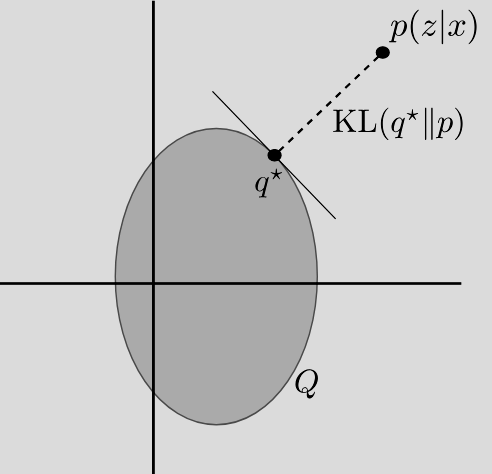
\includegraphics[width=8cm]{figures/VI.png}
    \end{center}
    \caption{Abstraction of the variational inference problem. We seek to find an approximate posterior distribution that minimizes the KL divergence. Figure credit: Jeffrey Regier}
\end{figure}
\begin{align*}
    q^*
    &= \underset{q \in Q}{\text{argmin}} \ \text{KL}(q(z)||p(z|x))\\
    &= \underset{q \in Q}{\text{argmin}} \ \ex{q}[log(q(z)) - log(p(z|x))]\\
    &= \underset{q \in Q}{\text{argmin}} \ \ex{q}[log(q(z)) - log(p(z,x))] + log(p(x))\\
    &= \underset{q \in Q}{\text{argmin}} \ \ex{q}[log(q(z)) - log(p(z,x))]\\
    &= \underset{q \in Q}{\text{argmin}} \ \ex{q}[log(q(z)) - log(p(x|z) - log(p(z)))]\\
    &= \underset{q \in Q}{\text{argmax}} \ \ex{q}[log(p(x|z))] - \text{KL}(q(z)||p(z)) = \text{ELBO}\\ 
\end{align*}
\begin{align*}
    \text{log } p(x) 
    &= \ex{q}[\text{log } p(x)] \\
    &= \ex{q}\left[\text{log } \frac{p(x|z)p(z)}{p(z|x)}\right] \\
    &= \ex{q}\left[\text{log } \left(\frac{p(x|z)p(z)}{p(z|x)} \times \frac{q(z)}{q(z)}\right) \right] \\
    &= \ex{q}[\text{log } p(x|z)] - \ex{q}\left[ \text{log } \frac{q(z)}{p(z)}\right] + \ex{q}\left[ \text{log } \frac{q(z)}{p(z|x)}\right] \\
    &= \ex{q}[\text{log } p(x|z)] - \text{KL} (q(z)||p(z)) +  \text{KL}(q(z)||p(z|x)) \\
    &= \text{ELBO} +  \text{KL}(q(z)||p(z|x))
\end{align*}


\subsection{}
\begin{align*}
    \psi, \theta = \psi, \theta -  \eta \nabla_{\psi, \theta} \sum_{i=1}^{N}\text{ELBO}(q_{\psi_i}, x_i, \theta)
\end{align*}



\subsection{}

\subsubsection*{Stochastic VI}
\begin{align*}
    \psi, \theta = \psi, \theta -  \eta \frac{N}{B} \nabla_{\psi, \theta} \sum_{i=1}^{B}\text{ELBO}(q_{\psi_i}, x_i, \theta)
\end{align*}

\subsubsection*{Amortized VI}
\begin{align*}
    \phi, \theta = \phi, \theta -  \eta \frac{N}{B} \nabla_{\phi, \theta} \sum_{i=1}^{B}\text{ELBO}(q_{\phi}(.|x_i), x_i, \theta)
\end{align*}


\subsection{}
\begin{align*}
    p_{\theta}(x|z) = \frac{1}{(\sqrt{2\pi} \sigma)^D} e ^ {-\frac{1}{2\sigma^2}||x - f_{\theta}(z)||^2} \\
    \text{log } p_{\theta}(x|z) = C - \frac{1}{2\sigma^2}||x - f_{\theta}(z)||^2
\end{align*}
where $D$ is the dimentionality of the $x$.
\begin{align*}
    \text{KL}(q(z)||p(z)) 
    &= \frac{1}{2}(tr(\text{diag}(\sigma_{\phi}^2(x))) + \mu_{\phi}(x)^T\mu_{\phi}(x) - k - \text{log } \text{det } \text{diag}(\sigma_{\phi}^2(x))) \\
    &= \frac{1}{2}\left(\text{sum}(\sigma_{\phi}^2(x)) + ||\mu_{\phi}(x)||^2 - k - \text{log mul}(\sigma_{\phi}^2(x))\right)
\end{align*}
where $k$ is the dimentionality of the $z$.
\begin{align*}
    L 
    &= -\ex{q}[\text{log } p(x|z)] + \text{KL} (q(z)||p(z)) \\
    &= \frac{1}{2\sigma^2}||x - f_{\theta}(z)||^2 + \frac{1}{2}\left(\text{sum}(\sigma_{\phi}^2(x)) + ||\mu_{\phi}(x)||^2 - k - \text{log mul}(\sigma_{\phi}^2(x))\right)
\end{align*}


\subsection{}
\begin{align*}
    \text{ELBO}
    &= - \text{KL}(q(z)||p(z|x))\\
    &= - \ex{q}[log(q(z)) - log(p(z|x))]\\
    &= - \ex{q}[log(q(z)) - log(p(z,x))] + log(p(x))\\
    &= - \ex{q}[log(q(z)) - log(p(z,x))]\\
    &= - \ex{\prod_{i} q_i(z_i)}[log(\prod_{i} q_i(z_i)) - log(p(z,x))]\\
    &= - \ex{\prod_{i} q_i(z_i)}[\sum_{i} log\  q_i(z_i) - log(p(z,x))]\\
    &= - \int \prod_{i} q_i(z_i)\left[\sum_{i} log\  q_i(z_i) + log(p(z,x))\right] dz \\
    &= - \int \left[\prod_{i} q_i(z_i)\right]\sum_{i} log\  q_i(z_i) dz + \int \left[\prod_{i} q_i(z_i)\right] log(p(z,x)) dz \\
    &= - \int q_j(z_j) \int \left[\prod_{i \neq j} q_i(z_i)\right]\sum_{i} log\  q_i(z_i) dz + \int q_j(z_j)\int \left[\prod_{i \neq j} q_i(z_i)\right] log(p(z,x)) dz \\
    &= - \int q_j(z_j) log \ q_j(z_j) \int \prod_{i \neq j} q_i(z_i)dz - \int q_j(z_j) \int \left[\prod_{i \neq j} q_i(z_i)\right]\sum_{i \neq j} log\  q_i(z_i) dz + \int q_j(z_j) \ex{z_{-j}}[log(p(z,x))]dz_j \\
    &= - \int q_j(z_j) log \ q_j(z_j) dz_j - \int \left[\prod_{i \neq j} q_i(z_i)\right]\sum_{i \neq j} log\  q_i(z_i) dz_{-j} + \int q_j(z_j) \ex{z_{-j}}[log(p(z,x))]dz_j \\
    &= - \int q_j(z_j) log \ q_j(z_j) dz_j + \int q_j(z_j) \ex{z_{-j}}[log(p(z,x))]dz_j + C\\
    &= - \int q_j(z_j) \left[log \ q_j(z_j) - \ex{z_{-j}}[log(p(z,x))]\right]dz_j + C\\
\end{align*}
\begin{align*}
    Lagrangian 
    &= - \int q_j(z_j) \left[log \ q_j(z_j) -  q_j(z_j) \ex{z_{-j}}[log(p(z,x))]\right]dz_j - \sum_{i} \lambda_i \int q_i(z_i)dz_i \\
    \frac{\partial Lagrangian}{\partial q_j} 
    &= \ex{z_{-j}}[log(p(z,x))] - log \ q_j(z_j)  - 1 - \lambda_j = 0 \\
    log \ q_j(z_j) 
    &= \ex{z_{-j}}[log(p(z,x))] + C \\
    q_j(z_j) 
    & \propto exp[{\ex{z_{-j}}[log \ p(z,x)]}]
\end{align*}


\section{Diffusion Models}

\subsection{}


\begin{align*}
    q(z_t|x) 
    &= \mathcal{N}(a_tx, \sigma_t^2I) \\
    &=a_tx + \mathcal{N}(0, \sigma_t^2I) \\
    &= Dist(0, a_t^2) + \mathcal{N}(0, \sigma_t^2I)\\
    \text{Var}_q &= a_t^2 + \sigma_t^2 = 1 \\
    a_t &= \sqrt{1 - \sigma_t^2}
\end{align*}


\subsection{}
\begin{align*}
    q(z_s, z_t|x) = q(z_s|z_t, x)q(z_t|x) = q(z_s|z_t)q(z_t|x)
\end{align*}


\subsection{}
\begin{align*}
    z_s &\sim \mathcal{N}(a_sx, \sigma_s^2 I) \\
    z_t &\sim \mathcal{N}(a_tx, \sigma_t^2 I) \\
    \frac{a_t}{a_s} z_s &\sim \mathcal{N}(a_tx, \frac{a_t^2}{a_s^2}\sigma_s^2 I) \\
    \mathcal{N}(0, (\sigma_t^2 - \frac{a_t^2}{a_s^2}\sigma_s^2)I) + \frac{a_t}{a_s} z_s &\sim \mathcal{N}(a_tx, \sigma_t^2I) \\
    \mathcal{N}(0, (\sigma_t^2 - \frac{a_t^2}{a_s^2}\sigma_s^2)I) + \frac{a_t}{a_s} z_s &\sim z_t \\
    \mathcal{N}(\frac{a_t}{a_s} z_s, (\sigma_t^2 - \frac{a_t^2}{a_s^2}\sigma_s^2)I) &\sim z_t \\
    \mathcal{N}(a_{t|s}z_s, \sigma_{t|s}^2I) &\sim z_t \\
\end{align*}
where,
\begin{align*}
    a_{t|s} = \frac{a_t}{a_s}, \ 
    \sigma_{t|s}^2 = (\sigma_t^2 - \frac{a_t^2}{a_s^2}\sigma_s^2)
\end{align*}


\subsection{}
\begin{align*} 
    q(z_s|z_t, x) 
    &\propto q(z_t|z_s)q(z_s|x) \\
    &\propto \mathcal{N}(a_{t|s}z_s, \sigma_{t|s}^2I) \mathcal{N}(a_{s}x, \sigma_{s}^2I) \\
    &\propto exp(-\frac{1}{2}(\frac{z_t - a_{t|s}z_s}{\sigma_{t|s}})^2 -\frac{1}{2}(\frac{z_s - a_sx}{\sigma_{s}})^2) \\
    &\propto exp(-\frac{1}{2}\frac{(\sigma_s^2a_{t|s}^2 + \sigma_{t|s}^2)z_s^2 + (z_ta_{t|s}\sigma_s^2 + a_sx\sigma_{t|s}^2)z_s}{\sigma_{t|s}^2\sigma_s^2}) \\
    &\propto exp(-\frac{1}{2}\frac{(\sigma_t^2)z_s^2 + (z_ta_{t|s}\sigma_s^2 + a_sx\sigma_{t|s}^2)z_s}{\sigma_{t|s}^2\sigma_s^2}) \\
    &\propto exp(-\frac{1}{2}\frac{z_s^2 + \frac{z_ta_{t|s}\sigma_s^2 + a_sx\sigma_{t|s}^2}{\sigma_t^2}z_s}{\frac{\sigma_{t|s}^2\sigma_s^2}{\sigma_t^2}}) \\
    &\propto exp(-\frac{1}{2}(\frac{z_s - \mu_Q(z_t, x; s, t)}{\sigma_Q^2(s, t)})^2) \\
    &\propto \mathcal{N}(\mu_Q(z_t, x; s, t), \sigma_Q^2(s, t)) 
\end{align*}
where,
\begin{align*}
    \mu_Q(z_t, x; s, t) &= \frac{(a_{t|s}\sigma_s^2)}{\sigma_t^2}z_t + \frac{(a_s\sigma_{t|s}^2)}{\sigma_t^2}x\\
    \sigma_Q^2(s, t) &= \frac{\sigma_{t|s}^2\sigma_s^2}{\sigma_t^2}
\end{align*}


\subsection{}
\begin{align*}
    D_{\text{KL}}(q(z_s|z_t, x) || p_{\theta}(z_s|z_t)) 
    &= \frac{1}{2}(d + \frac{1}{\sigma_Q^2(s, t)}||\mu_Q(z_t, x; s, t) - \mu_{\theta}(z_t;s, t)||_2^2 - d + \text{log} (1)) \\
    &= \frac{1}{2\sigma_Q^2(s, t)}||\mu_Q(z_t, x; s, t) - \mu_{\theta}(z_t;s, t)||_2^2\\
\end{align*}


\subsection{}
\begin{align*}
    D_{\text{KL}}(q(z_s|z_t, x) || p_{\theta}(z_s|z_t)) 
    &=\frac{1}{2\sigma_Q(s, t)}||\mu_Q(z_t, x; s, t) - \mu_{\theta}(z_t;s, t)||_2^2\\
    &=\frac{1}{2\sigma_Q(s, t)}||\frac{(a_{t|s\sigma_s^2})}{\sigma_t^2}z_t +  \frac{(a_s\sigma_{t|s}^2)}{\sigma_t^2}x - \frac{(a_{t|s\sigma_s^2})}{\sigma_t^2}z_t +  \frac{(a_s\sigma_{t|s}^2)}{\sigma_t^2}\hat{x}_{\theta}(z_t, t) ||_2^2\\
    &=\frac{(a_s^2\sigma_{t|s}^4)}{2\sigma_t^4\sigma_Q^2(s, t)}||x - \hat{x}_{\theta}(z_t, t) ||_2^2\\
    &=\frac{1}{2}\gamma||x - \hat{x}_{\theta}(z_t, t) ||_2^2\\
\end{align*}
where,
\begin{align*}
    \gamma 
    &= \frac{a_s^2\sigma_{t|s}^4}{\sigma_t^4\sigma_Q^2(s, t)} \\
    &= \frac{a_s^2\sigma_{t|s}^2}{\sigma_t^2\sigma_s^2} \\
    &= \frac{a_s^2(\sigma_t^2 - \frac{a_t^2}{a_s^2}\sigma_s^2)}{\sigma_t^2\sigma_s^2} \\
    &= \frac{a_s^@\sigma_t^2 - a_t^2\sigma_s^2}{\sigma_t^2\sigma_s^2} \\
    &= \frac{a_s^2}{\sigma_s^2} - \frac{a_t^2}{\sigma_t^2}\\
    &= \text{SNR}(s) - \text{SNR}(t)
\end{align*}

\subsection{}
\begin{align*}
    L_{\infty}(x) 
    &= \underset{T\to \infty}{\text{lim}} L_{T}(x) \\
    &=\underset{T\to \infty}{\text{lim}} \frac{T}{2}\ex{}[(SNR(s(i)) - SNR(t(i)))||x-\hat{x}_{\theta}(z_{t(i)};t(i))||_2^2] \\
    &=\underset{T\to \infty}{\text{lim}} \frac{T}{2}\ex{}[(SNR(t - \frac{1}{T}) - SNR(t))||x-\hat{x}_{\theta}(z_{t(i)};t(i))||_2^2] \\
    &= -\frac{1}{2}\ex{}[\underset{T\to \infty}{\text{lim}}T(SNR(t) - SNR(t - \frac{1}{T}))||x-\hat{x}_{\theta}(z_{t(i)};t(i))||_2^2] \\
    &= -\frac{1}{2}\ex{}[SNR'(t)||x-\hat{x}_{\theta}(z_{t(i)};t(i))||_2^2] \\
\end{align*}


\section{Score Matching}
\subsection{}
\begin{align*}
    x_{t+1} &= x_{t} + \delta \nabla_x \text{log } p(x_t) \\
    \text{No Update: } x_t &= x_t + \delta \nabla_x \text{log } p(x_t) \\
    \nabla_x \text{log } p(x_t) &= 0
\end{align*}
At point $x_t$, $p(x)$ reaches a peak because the gradient is zero at this location.

Maximum likelihood typically identifies the global maximum, whereas this method may converge on a local maximum.


\subsection{}
There are two reasons for the presence of a noise term. First, it helps the 
algorithm escape local maxima, especially if the starting point is close to 
one. Second, the noise encourages the discovery of flatter maxima.

\subsection{}
\begin{align*}
    \nabla_x \text{log} q(x) 
    &= \frac{q'(x)}{q(x)} = \frac{\frac{1}{M}\sum_{i=1}^M \frac{-2(x - x^{(i)})}{2\sigma^2}K(x|x^{(i)})}{\frac{1}{M}\sum_{i=1}^M K(x|x^{(i)})} \\
    &= \frac{q'(x)}{q(x)} = \frac{\sum_{i=1}^M \frac{1}{\sigma^2}(x^{(i)} - x)K(x|x^{(i)})}{\sum_{i=1}^M K(x|x^{(i)})} \\
\end{align*}


\subsection{}
If we lack sufficient data in a particular region, this method will not 
produce an accurate density estimate for that area, which may prevent us 
from correctly identifying the peak of the density.


\subsection{}
\begin{align*}
    J_1(\theta) = \ex{q(x)}[\frac{1}{2}||s_{\theta}(x)||^2] - g(\theta) + C
\end{align*}

\begin{align*}
    g(\theta) 
    &= \ex{q(x)}[\left< s(x), \frac{\partial \text{log }q(x)}{\partial x}\right>]\\
    &= \int_x q(x)\left< s(x), \frac{\partial \text{log }q(x)}{\partial x}\right> dx\\
    &= \int_x q(x)\left< s(x), \frac{\frac{\partial q(x)}{\partial x}}{q(x)}\right> dx\\
    &= \int_x \left< s(x), \frac{\partial q(x)}{\partial x}\right> dx\\
    &= \int_x \left< s(x), \frac{\partial}{\partial x}\int_{x_0} q_0(x_0)q(x|x_0)dx_0\right> dx\\
    &= \int_x \left< s(x), \int_{x_0} q_0(x_0)\frac{\partial q(x|x_0)}{\partial x}dx_0\right> dx\\
    &= \int_x \left< s(x), \int_{x_0} q_0(x_0)q(x|x_0)\frac{\partial \text{log } q(x|x_0)}{\partial x}dx_0\right> dx\\
    &= \int_x \int_{x_0} q_0(x_0)q(x|x_0) \left< s(x), \frac{\partial \text{log } q(x|x_0)}{\partial x}\right> dxdx_0\\
    &= \int_x \int_{x_0} q(x,x_0) \left< s(x), \frac{\partial \text{log } q(x|x_0)}{\partial x}\right> dxdx_0\\
    &= \ex{q(x,x_0)}\left[\left< s(x), \frac{\partial \text{log } q(x|x_0)}{\partial x}\right>\right]\\
\end{align*}
So,
\begin{align*}
    J_1(\theta) = J_2(\theta) + C
\end{align*}
\subsection{}
\begin{align*}
    J_2(\theta) 
    &= \ex{q(x,x_0)}[\frac{1}{2}||s_{\theta}(x) - \nabla_x \text{log } q(x|x_0)||^2]\\
    &= \ex{q(x,x_0)}[\frac{1}{2}||s_{\theta}(x) - \frac{1}{\sigma^2}(x- x_0)||^2]\\
\end{align*}

\begin{algorithm}
    \caption{Diffusion Training}
    \begin{algorithmic}[1]
        \For{$i \gets 1$ to $m$}
            \State $x_1 = x^{(i)}$
            \For{$t \gets 1$ to $T$}
                \State $x_{t+1} = x_t + \lambda s_{\theta}(x_t) + \sqrt{2\lambda}\epsilon$
                \State $\theta = \theta - \eta \nabla_\theta J_2(\theta)$ 
            \EndFor
        \EndFor
    \end{algorithmic}
\end{algorithm}

\begin{algorithm}
    \caption{Diffusion Evaluating}
    \begin{algorithmic}[1]
        \State $x_1 \sim \mathcal{N}(0, I)$
        \For{$t \gets 1$ to $T$}
            \State $x_{t+1} = x_t + \lambda s_{\theta}(x_t) + \sqrt{2\lambda}\epsilon$
            \State $\theta = \theta - \eta \nabla_\theta J_2(\theta)$ 
        \EndFor
        \State \Return $x_T$
    \end{algorithmic}
\end{algorithm}


% \section{Stability Analysis of GAN}


\end{document}

